\section{Linear Systems}
A linear system is a problem defined as follows: given $A \in \RR^{n \times n},\,b \in \RR^n$ we want to find, if possible, $x \in \RR^n$ such that $Ax = b$.

\subsection{Solvability}
If we consider $a^{(i)}$ the $i$-th column of matrix $A$, we can express the linear system as:
\begin{dmath*}
	Ax = a^{(1)}x_1 + a^{(2)}x_2 + \ldots + a^{(n)}x_n \stackrel{!}{=} b
\end{dmath*}

So a solution exists iff $b$ can be represented as a linear combination of columns of $A$, i.e. $b \in \op{span}(a^{(1)},\ldots,a^{(n)})$.
We already know that if $A$ has \emph{full-rank}\footnote{Its rank is the same as its dimension.}, then
\begin{equation*}
	\op{null}(A) \definedas \{ x \in \RR^n | Ax = 0 \} = \{0\}
\end{equation*}
so, by Grassmann's formula, $\op{dim}(Im(A)) = n$, therefore $b \in \op{span}(a^{(1)},\ldots,a^{(n)})$.

From now on, we will typically assume $A$ to be full rank.

\paragraph{How to compute a solution}
\todo{This is actually nonsensicle here, we should move it to where we actually talk about solving.}We may be tempted to proceed the naive way: $Ax = b \implies x = A^{-1}b$, but this turns out to be a very bad idea because:
\begin{itemize}
	\item Inverting a matrix in practice requires solving $n$ linear systems of the form $Ax = e_i$.
	\item Matrix inversion can be unstable.
\end{itemize}

\subsection{Conditioning of linear systems}
Let's see a simple $2 \times 2$ linear system, to get an idea on why resolution of linear system can be well or badly conditioned to different degrees. Consider:
\begin{align*}
	\begin{cases}
		a_{11} x_1 + a_{12} x_2 &= b_1 \\
		a_{21} x_1 + a_{22} x_2 &= b_2
	\end{cases}
\end{align*}
In the ideal world, the solution of each equation is a mono-dimensional sub-space, i.e. a line. If we look at the intersection of these two lines, which is the combined solution of the linear system, we get a single point (a null-dimensional space).

However, if we take into account representation error on both $b$ and $A$, we get that the solution to each equation is not just a line, but more like a strip. That is, all the possible lines which are near enough the theoretical solution to be rounded (in some sense) to it are possible solutions.
\begin{figure}[H]
	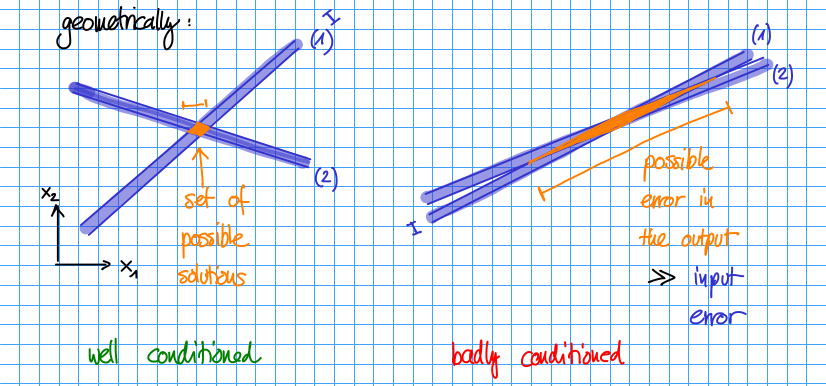
\includegraphics[width=\textwidth]{linSysConditioning}
\end{figure}
If we now consider the intersection of these two strips, we get an entire patch of the plane as possible solution set. We can see how the extent of this patch grows considerably the more the two solution strips tend to be parallel. This is, in simple terms, the idea behind the conditioning of a linear system.

\paragraph{Condition number of a linear system}
The general problem associated to solving the linear system $Ax = b$ is:
\begin{equation*}
	(A, b) \mapsto x = A^{-1} b
\end{equation*}
We want to simplify it and make it a mono-variate problem, so we choose to fix "b" as exact and to just consider $A$ as an input which may be perturbed. So we have the problem:
\begin{equation*}
	A \mapsto x = A^{-1} b
\end{equation*}
We consider an input error
\begin{equation}\label{eq:error}
{
	E \definedas \tilde{A} - A \st ||E|| \leq \eps||A|| \tag{\ensuremath{\circ}}
}
\end{equation}
and we get output error:
\begin{equation*}
	\tilde{x} - x = \tilde{A}^{-1} b - \tilde{A}^{-1} b
\end{equation*}
For estimating the output error we consider:
\begin{align*}
	Ax &= \tilde{A} \tilde{x} = b\\
	Ax &= (A+E) \tilde{x} = A \tilde{x} + E \tilde{x}\\
	Ax - A \tilde{x} &= E \tilde{x}\\
	A(x - \tilde{x}) &= E \tilde{x}\\
	\implies x - \tilde{x} &= A^{-1} E \tilde{x}\\
\end{align*}
So in norm we have:
\begin{dmath*}
	||x-\tilde{x}||\, = ||A^{-1} E x|| \stackrel{\scriptsize{\eqref{prop:indnorm1}}}{\leq} ||A^{-1}E||\,||x|| \stackrel{\scriptsize{\eqref{prop:indnorm2}}}{\leq} ||A^{-1}E||\,||E||\,||x||
\end{dmath*}{
\begin{dmath*}
	\frac{||x - \tilde{x}||}{x} \leq ||A^{-1}||\,||E|| \stackrel{\scriptsize{\eqref{eq:error}}}{\leq} \underbrace{||A^{-1}||\,||A||}_{=: \kappa(A)}\,\eps
\end{dmath*}
So we have obtained an upper bound on the error, $\kappa(A) \definedas ||A^{-1}||\,||A||$, which is defined as the \emph{condition number of matrix} $A$.
\begin{Rem}
	This condition number has a very nice geometrical interpretation, since it corresponds, in the matrix space, to the distance between $A$ and the sungular subspace\footnote{Subspace of matrices $M$ such that $\op{det}(M) = 0$.}. So the higher the condition number, the closer is $A$ to be singular.
\end{Rem}

\subsection{A posteriori error analysis}
With the condition number we get an upper bound on the error, but even when we get a bad $\kappa$ from our analysis, our problem may behave unexpectedly well. In fact $\kappa$ gives us an upper bound, but nothing prevents the solution to show a lower error. Is there a way to get an \emph{estimate} on the actual error we are going to get?

\paragraph{Going backward}
The idea is to perform what is called a \emph{backward} or \emph{a posteriori} error analysis.
We solve $Ax = b$ and we get some $\tilde{x}$ coming with its error. Now we change perspective and we consider $\tilde{x}$ to be the exact solution of a perturbed problem $\tilde{A}$. So we have:
\begin{align*}
	Ax &= b\\
	\tilde{A} \tilde{x} &= b, \quad \tilde{A} = A + E
\end{align*}
where $E$ is unknown.

Why should this be helpful?\\
Because we are pushing the output error into a form of input one. We are now asking \enquote{What is the smallest perturbation $E$ for which $\tilde{A} \tilde{x} = b$?}
\begin{Teo}[Wilkinson]
	\begin{align*}
		\omega \definedas& min \left\{ \frac{||E||}{||A||} \tc (A + E)\,\tilde{x} = b \right\}\\
		=& \frac{||\tau||}{||A||\,||\tilde{x}||}
	\end{align*}
	where $\tau = A\tilde{x} - b$ is called the \emph{residual} of the linear system and $\omega$ is called the \emph{backward error} of $\tilde{x}$.
\end{Teo}
Then the (forward) output error can be \emph{estimated} by:
\begin{equation*}
	\frac{||x - \tilde{x}||}{||\tilde{x}||} \approx \kappa(A) \cdot \omega
\end{equation*}

\begin{figure}[H]
	\begin{matlabtip}
		\small{
		In Matlab $Ax = b$ can be solved by using the backslash operator:
		\begin{lstlisting}[aboveskip=1mm, belowskip=1.5mm]
			x = A\b;
		\end{lstlisting}
		The condition number $\kappa(A)$ can be computed with:
		\begin{lstlisting}[aboveskip=1mm, belowskip=1.5mm]
			cond(A)
		\end{lstlisting}
		The norm is simply:
		\begin{lstlisting}[aboveskip=1mm, belowskip=1.5mm]
			norm(A)
		\end{lstlisting}
		}
	\end{matlabtip}
\end{figure}

\subsection{Gaussian elimination}
We now start to see methods for solving linear systems.

\paragraph{Triangular systems}
The easiest system we can solve is a triangular one, i.e. one represented by a triangular matrix.

A lower triangular system can be solved using \emph{forward substitution}: since the system is lower triangular, the first unknown $x_1$ can be computed directly and substituted in all the following equations; then $x_2$ can be directly computed and substituted in all the following, and so on.

If we count how many \emph{flop}\footnote{flop = floating point operations} are required for the forward substitution algorithm, we get
\begin{equation*}
	2\,j - 1
\end{equation*}
for the $j$-th step, summing up to a total of
\begin{equation*}
	\sum_{j=1}^{n} 2\,j - 1 = n^2
\end{equation*}
where $n$ is the order of the matrix. So forward substitution scales quadratically with matrix order.

\paragraph{Gaussian elimination}
Since we know how to solve a triangular system, the purpose of gaussian elimination is to bring a generic system into a triangular form.

\begin{figure}[h]
	\begin{matlabtip}
		\small{
		A lower triangular matrix can be \emph{extracted} from an existing general matrix $A$:
		\begin{lstlisting}[aboveskip=1mm, belowskip=1.5mm]
			tril(A)
		\end{lstlisting}
		An upper triangular can instead be extracted with:
		\begin{lstlisting}[aboveskip=1mm, belowskip=1.5mm]
			triu(A)
		\end{lstlisting}
		How a matrix looks like, qualitatively, can be checked with:
		\begin{lstlisting}[aboveskip=1mm, belowskip=1.5mm]
			spy(A)
		\end{lstlisting}
		}
	\end{matlabtip}
\end{figure}

% EOF
 